\chapter{Conics}

\section{Group Laws on Conics}

Consider a conic section $\mathcal{C}$ and a point $O \in \mathcal{C}$. For any points $P,Q \in \mathcal{C}$,
let $\ell'$ be the line passing through $O$ such that $\ell' \parallel \ell$ where
$\ell$ is the line joining $P$ and $Q$. If $\ell'$ intersects $\mathcal{C}$ at a point
other than $O$, call that point $R$. Otherwise, take $R=O$. Define a binary
operation $\oplus : \mathcal{C} \times \mathcal{C} \to \mathcal{C}$ as $P \oplus Q := R$.
\vspace{1ex}

\begin{figure}[H]
    \center
    \begin{tikzpicture}
        \tkzDefPoint(0,0){C}
        \tkzDefPoint(-2,0){O}
        \tkzDefPoint({2*cos(70*pi/180)},{2*sin(70*pi/180)}){P}
        \tkzDefPoint({2*cos(-30*pi/180)},{2*sin(-30*pi/180)}){Q}
        \tkzDefPoint({2*cos(-140*pi/180)},{2*sin(-140*pi/180)}){R}

        \tkzDrawPoints[fill=black](O,P,Q,R)
        \tkzDrawLine[<->,line width=0.5,add=0.2 and 0.2](P,Q)
        \tkzDrawLine[<->,line width=0.5,add=0.5 and 0.5](O,R)
        \tkzDrawCircle[color=black,line width=0.5](C,O)

        \tkzLabelPoints[left](O)
        \tkzLabelPoints[above right](P)
        \tkzLabelPoints[right](Q)
        \tkzLabelPoints[below left](R)

        \tkzLabelLine[pos=1.3](P,Q){$\ell$}
        \tkzLabelLine[pos=1.7](O,R){$\ell'$}
    \end{tikzpicture}

    \caption{$P \oplus Q$ when $\mathcal{C}$ is a circle.}
\end{figure}

We'll first find formulae to calculate $P \oplus Q$ and then proceed to prove
that $\mathcal{C}$ is a group with $\oplus$.

\subsection*{Ellipse}

\begin{wrapfigure}{r}{0.3\textwidth}
    \centering
    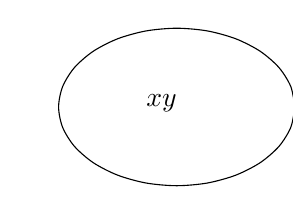
\begin{tikzpicture}
        \tkzDefPoint(-1.5,0){X'}
        \tkzDefPoint(1.5,0){X}
        \tkzDefPoint(0,1){Y}
        \tkzDefPoint(0,-1){Y'}

        \tkzDrawLine[<->,line width=0.5,add=0.1 and 0.1](X,X')
        \tkzDrawLine[<->,line width=0.5,add=0.2 and 0.2](Y,Y')

        \tkzLabelLine[pos=-0.15](X,X'){$x$}
        \tkzLabelLine[pos=-0.3](Y,Y'){$y$}

        \draw[domain=0:360,smooth,variable=\t] plot ({1.5*cos(\t},{1*sin(\t)});
    \end{tikzpicture}

    \caption{}
\end{wrapfigure}

If $\mathcal{C}$ is an ellipse, consider a coordinate system centred at the centre of the
ellipse with its major and minor axes as $x$ and $y$ axes respectively as shown in
the figure on the right. Its equation will be
$a^{-2} x^2 + b^{-2} y^2 = 1$ in this coordinate system where
$a,b\in\mathbb{R}^+$ . Any point $P \in \mathcal{C}$ has coordinates
$(a \cos \theta, b \sin \theta)$ where $\theta \in [0,2\pi)$ is the angle $P$
forms with the positive $x$-axis in the counter-clockwise direction.
\vspace{1ex}

Consider points $P,Q,R \in \mathcal{C}$ such that $P \oplus Q = R$ and they form angles
$\theta_1$, $\theta_2$ and $\theta_3$ w.r.t. $x$-axis respectively. Also, let
$\theta_0$ be the angle formed by $O$ w.r.t. positive $x$-axis.
\vspace{1ex}

\noindent
Since $P \oplus Q = R$, we have $OR \parallel PQ$ and hence slope of $OR$ and $PQ$
will be the same. Using their coordinates, this can be written as,
\[
    \frac{b \sin \theta_3 - b \sin \theta_0}{a \cos \theta_3 - a \cos \theta_0}
    = \frac{b \sin \theta_2 - b \sin \theta_1}{a \cos \theta_2 - a \cos \theta_1}
\]
We can cancel out $b/a$ on both sides. After cross-multiplying and grouping the
terms with the same pair of angles, we get
\[
    \sin(\theta_3 - \theta_2) + \sin(\theta_1 - \theta_3)
    = \sin(\theta_0 - \theta_2) + \sin(\theta_1 - \theta_0)
\]
Using the trigonometric identity
$\sin x + \sin y = 2 \sin\frac{x+y}{2}\cos\frac{x-y}{2}$, this further simplifies
\[
    2\sin\left(\frac{\theta_1 - \theta_2}{2}\right)\cos\left(\frac{\theta_1 + \theta_2 - 2\theta_3}{2}\right)
    = 2\sin\left(\frac{\theta_1 - \theta_2}{2}\right)\cos\left(\frac{\theta_1 + \theta_2 - 2\theta_0}{2}\right)
\]
If $P \neq Q$, then $\theta_1 \neq \theta_2$. So, $\sin$ won't be zero and hence, we
can cancel the $2$ and $\sin$, leaving the following relation between the
arguments of $\cos$,
\[
    \frac{\theta_1 + \theta_2}{2} - \theta_3
    = 2n\pi \pm \frac{\theta_1 + \theta_2 - 2\theta_0}{2}
\]
As shifts of $2n\pi$ don't affect $\theta_3$, we can ignore that term on the RHS.
The positive case results in $\theta_3 = \theta_0$ but this just indicates the
point $O$ which we know already lies on $\ell'$ and $\mathcal{C}$. The negative case
gives $\theta_3 = \theta_1 + \theta_2 - \theta_0$.
\vspace{1ex}

\noindent
If $P=Q$, then $\theta_1 = \theta_2$. In this case, the slope of line $PQ$ will be
the slope of the tangent at $P$. Equating slope of tangent at $P$ with slope of
$OR$,
\[
    -\frac{b}{a}\cot\theta_1
    = \frac{b \sin \theta_3 - b \sin \theta_0}{a \cos \theta_3 - a \cos \theta_0}
\]
Again cancelling out $b/a$ from both sides, cross multiplying and grouping terms
with same pairs of angles, we obtain,
\[
    \cos\theta_1\cos\theta_0 + \sin\theta_1\sin\theta_0
    = \cos\theta_1\cos\theta_3 + \sin\theta_1\sin\theta_3
\]
The LHS and RHS are just $\cos(\theta_0 - \theta_1)$ and $\cos(\theta_3-\theta_1)$
respectively. Thus we obtain the following relation for the arguments,
\[
    \theta_3 - \theta_1 = 2n\pi \pm (\theta_0 - \theta_1)
\]
Again, we can ignore shifts by $2n\pi$. The positive case results in
$\theta_3 = \theta_0$ which just indicates point $O$ lying on $\ell'$. The
negative case gives $\theta_3 = 2\theta_1 - \theta_0$ which matches the formula
we obtained for $P \neq Q$ case when $\theta_1 = \theta_2$.
\vspace{1ex}

Thus for any $P,Q \in \mathcal{C}$ with parameters $\theta_1$ and $\theta_2$ respectively
for an ellipse $\mathcal{C}$, $P \oplus Q = R$ has parameter
$\theta_3 = \theta_1 + \theta_2 - \theta_0$ where $t_0$ is the parameter for point
$O$. Note that we always add or subtract multiples of $2\pi$ to make sure
$\theta_3 \in [0,2\pi)$.
\vspace{1ex}

It is easy to see that $\oplus$ satisfies closure for $\mathcal{C}$. We'll verfiy each of 
the group axioms now.

\begin{enumerate}
    \item{\textbf{Identity:}} For any $P \in \mathcal{C}$ with parameter $\theta$,
        $P \oplus O$ will have parameter
        $\theta' = \theta + \theta_0 - \theta_0 = \theta$. Thus $O$ acts as the
        identity element for $\oplus$.

    \item{\textbf{Inverse:}} The point $Q$ with parameter $2\theta_0 - \theta$
        gives the parameter of $P \oplus Q$ to be
        $\theta' = \theta + 2\theta_0 - \theta - \theta_0=\theta_0$. Hence, $Q$
        is the inverse of $P$.

    \item{\textbf{Associativity:}} For any $P,Q,R \in \mathcal{C}$ with parameters\
        $\theta_1$, $\theta_2$ and $\theta_3$ respectively, $P\oplus(Q \oplus R)$
        has parameter $\theta_1 + (\theta_2 + \theta_3 - \theta_0) - \theta_0$ or
        $\theta_1 + \theta_2 + \theta_3 - 2\theta_0$. On the other hand,
        $(P \oplus Q)\oplus R$ has parameter
        $(\theta_1 + \theta_2 - \theta_0) + \theta_3 - \theta_0$ or
        $\theta_1 + \theta_2 + \theta_3 - 2\theta_0$. Thus $\oplus$ is
        associative.
\end{enumerate}

\noindent
This shows that $\mathcal{C}$ is a group with $\oplus$ for the case where $\mathcal{C}$ is an ellipse.

\begin{theorem}
    If $\mathcal{C}$ is an ellipse,
    $\langle \mathcal{C},\oplus \rangle \cong \langle S^1,\cdot \rangle$ where
    $S^1=\{e^{i\theta}\in\mathbb{C}: \theta \in [0,2\pi)\}$.
\end{theorem}

\begin{proof}
    Consider $\varphi:\mathcal{C} \to S^1$ given by
    $\varphi((a\cos\theta,b\sin\theta)) = e^{i(\theta-\theta_0)}$. For any points
    $P,Q\in\mathcal{C}$ parametrized by $\theta_1$ and $\theta_2$ respectively,
    $P \oplus Q$ has parameter $\theta_1 + \theta_2 - \theta_0$. So,
    \[
        \varphi(P \oplus Q) = e^{i(\theta_1 + \theta_2 - 2\theta_0)}
        = e^{i(\theta_1 - \theta_0)}e^{i(\theta_2 - \theta_0)} = \varphi(P)\varphi(Q)
    \]
    Thus $\varphi$ is a homomorphism.
    \vspace{1ex}

    \noindent
    If $\phi(P)=\phi(Q)$ for some $P,Q\in\mathcal{C}$ parametrized by $\theta_1$
    and $\theta_2$ respectively, then
    \begin{align*}
        e^{i(\theta_1-\theta_0)} = e^{i(\theta_2-\theta_0)}
        \implies e^{i\theta_1}e^{i\theta_0} = e^{i\theta_2}e^{i\theta_0}
        \implies e^{i\theta_1} = e^{i\theta_2}
        \implies \theta_1 = 2n\pi + \theta_2
    \end{align*}
    i.e. $P=Q$. Thus $\varphi$ is injective.
    \vspace{1ex}

    \noindent
    For any $e^{i\theta} \in S^1$, we have the point
    $P=(a\cos(\theta+\theta_0),b\sin(\theta+\theta_0)) \in \mathcal{C}$ such that
    \[ \varphi(P) = e^{i(\theta + \theta_0 - \theta_0)} = e^{i\theta} \]
    Thus $\varphi$ is surjective. This shows that $\varphi$ is a bijective
    homomorphism i.e. an isomorphism from $\langle \mathcal{C},\oplus \rangle$ to
    $\langle S^1,\cdot \rangle$.
\end{proof}

\subsection*{Parabola}

\begin{wrapfigure}{r}{0.4\textwidth}
    \centering
    \begin{tikzpicture}[domain=-1.5:1.5]
        \tkzDefPoint(-1.5,0){X'}
        \tkzDefPoint(1.5,0){X}
        \tkzDefPoint(0,2.25){Y}
        \tkzDefPoint(0,0){Y'}

        \tkzDrawLine[<->,line width=0.5,add=0.1 and 0.1](X,X')
        \tkzDrawLine[<->,line width=0.5,add=0.2 and 0.3](Y,Y')

        \tkzLabelLine[pos=-0.15](X,X'){$x$}
        \tkzLabelLine[pos=-0.3](Y,Y'){$y$}

        \draw[smooth,variable=\t] plot ({\t},{pow(\t,2)});
    \end{tikzpicture}

    \caption{}
\end{wrapfigure}

If $\mathcal{C}$ is a parabola, consider a coordinate system with vertex of
$\mathcal{C}$ as origin, $x$-axis as tangent at vertex and $y$-axis perpendicular
to it as shown in the figure on the right. The equation of $\mathcal{C}$ in this
coordinate system will be $x^2=4ay$ where $a\in\mathbb{R}^+$. Any point on it can
be parametrized as $(2at,at^2)$ where $t \in \mathbb{R}$.
\vspace{1ex}

Let $O$, $P$, $Q$ and $R$ be points with parameters $t_0$, $t_1$, $t_2$ and $t_3$
respectively such that $P \oplus Q = R$. By definition of $P \oplus Q$, we have
$PQ \parallel OR$. Note that if $P=Q$, then slope at $P$ is
\[
    y'|_{x=2at_1} = \left(\frac{x}{2a}\right)_{x=2at_1}
    =t_1=\frac{t_1 + t_2}{2}
\]
and if $P \neq Q$, then $t_1 \neq t_2$ and slope of $PQ$ is 
\[
    \frac{at_2^2-at_1^2}{2at_2-2at_1} = \frac{t_1 + t_2}{2}
\]
So, we don't need to consider points being same as a separate case. Equating
slopes of $PQ$ and $OR$, we get,
\[ \frac{t_1 + t_2}{2} = \frac{t_0 + t_3}{2} \implies t_3 = t_1 + t_2 - t_0 \]

Thus, for any points $P,Q \in \mathcal{C}$ with parameters $t_1$ and $t_2$
respectively for a parabola $\mathcal{C}$, $P \oplus Q = R$ has parameter
$t_3 = t_1 + t_2 - t_0$ where $t_0$ is the parameter for point $O$.
\vspace{1ex}

It is easy to see that $\oplus$ satisfies closure for $\mathcal{C}$. We'll verfiy each of 
the group axioms now.

\begin{enumerate}
    \item{\textbf{Identity:}} For any $P \in \mathcal{C}$ with parameter $t$,
        $P \oplus O$ will have parameter $t' = t + t_0 - t_0 = t$. Thus $O$ acts
        as the identity element for $\oplus$.

    \item{\textbf{Inverse:}} The point $Q$ with parameter $2t_0 - t$ gives the
        parameter of $P \oplus Q$ to be $t' = t + 2t_0 - t - t_0 = t_0$. Hence,
        $Q$ is the inverse of $P$.

    \item{\textbf{Associativity:}} For any $P,Q,R \in \mathcal{C}$ with parameters
        $t_1$, $t_2$ and $t_3$ respectively, $P\oplus(Q \oplus R)$ has parameter
        $t_1 + (t_2 + t_3 - t_0) - t_0$ or $t_1 + t_2 + t_3 - 2t_0$. On the other
        hand, $(P \oplus Q)\oplus R$ has parameter $(t_1 + t_2 - t_0) + t_3 - t_0$
        or $t_1 + t_2 + t_3 - 2t_0$. Thus $\oplus$ is associative.
\end{enumerate}

\noindent
This shows that $\mathcal{C}$ is a group with $\oplus$ for the case where $\mathcal{C}$ is an
parabola.

\begin{theorem}
    If $\mathcal{C}$ is a parabola,
    $\langle \mathcal{C},\oplus \rangle \cong \langle \mathbb{R},+ \rangle$.
\end{theorem}

\begin{proof}
    Consider $\varphi:\mathcal{C} \to \mathbb{R}$ given by
    $\varphi((2at,at^2)) = t - t_0$. For any points
    $P,Q\in\mathcal{C}$ parametrized by $t_1$ and $t_2$ respectively,
    $P \oplus Q$ has parameter $t_1 + t_2 - t_0$. So,
    \[
        \varphi(P \oplus Q) = t_1 + t_2 - 2t_0 = (t_1 - t_0) + (t_2 - t_0)
        = \varphi(P) + \varphi(Q)
    \]
    Thus $\varphi$ is a homomorphism.
    \vspace{1ex}

    \noindent
    If $\phi(P)=\phi(Q)$ for some $P,Q\in\mathcal{C}$ parametrized by $t_1$ and
    $t_2$ respectively, then
    \begin{align*}
        t_1 - t_0 = t_2 - t_0 \implies t_1 = t_2
    \end{align*}
    i.e. $P=Q$. Thus $\varphi$ is injective.
    \vspace{1ex}

    \noindent
    For any $t \in \mathbb{R}$, we have the point
    $P=(2a(t + t_0),a(t + t_0)^2) \in \mathcal{C}$ such that
    \[ \varphi(P) = t + t_0 - t_0 = t \]
    Thus $\varphi$ is surjective. This shows that $\varphi$ is a bijective
    homomorphism i.e. an isomorphism from $\langle \mathcal{C},\oplus \rangle$ to
    $\langle \mathbb{R},+ \rangle$.
\end{proof}

\subsection*{Hyperbola}

\begin{wrapfigure}{r}{0.4\textwidth}
    \centering
    \begin{tikzpicture}
        \tkzDefPoint(-1.6,0){X'}
        \tkzDefPoint(1.6,0){X}
        \tkzDefPoint(0,1.6){Y}
        \tkzDefPoint(0,-1.6){Y'}

        \tkzDrawLine[<->,line width=0.5](X,X')
        \tkzDrawLine[<->,line width=0.5](Y,Y')

        \tkzLabelLine[pos=-0.3](X,X'){$x$}
        \tkzLabelLine[pos=-0.3](Y,Y'){$y$}

        \draw[domain=-2:{-3/24},smooth,variable=\t] plot ({\t},{0.25/\t});
        \draw[domain={3/24}:2,smooth,variable=\t] plot ({\t},{0.25/\t});
    \end{tikzpicture}

    \caption{}
\end{wrapfigure}

If $\mathcal{C}$ is a rectangular hyperbola, consider a coordinate system with
centre of $\mathcal{C}$ as origin and the asymptotes as $x$ and $y$ axes as shown
in the figure on the right. The equation of $\mathcal{C}$ in this coordinate
system will be $xy=c^2$ where $c \in \mathbb{R}^+$. Any point on it can be
parametrized as $(ct,ct^{-1})$ where $t \in \mathbb{R}^\times$.
\vspace{1ex}

Let $O$, $P$, $Q$ and $R$ be points with parameters $t_0$, $t_1$, $t_2$ and $t_3$
respectively such that $P \oplus Q = R$. By definition of $P \oplus Q$, we have
$PQ \parallel OR$. Note that if $P=Q$, then slope at $P$ is
\[
    y'|_{x=ct_1} = \left(-\frac{c^2}{x^2}\right)_{x=ct_1}
    = -\frac{1}{t_1^2} = -\frac{1}{t_1 t_2}
\]
and if $P \neq Q$, then $t_1 \neq t_2$ and slope of $PQ$ is 
\[
    \frac{ct_2^{-1}-ct_1^{-1}}{ct_2-ct_1} = \frac{t_1 - t_2}{t_1 t_2 (t_2 - t_1)}
    = -\frac{1}{t_1 t_2}
\]
So, we don't need to consider points being same as a separate case. Equating
slopes of $PQ$ and $OR$, we get,
\[ -\frac{1}{t_1 t_2} = -\frac{1}{t_0 t_3} \implies t_3 = \frac{t_1 t_2}{t_0} \]

Thus, for any points $P,Q \in \mathcal{C}$ with parameters $t_1$ and $t_2$
respectively for a rectangular hyperbola $\mathcal{C}$, $P \oplus Q = R$ has
parameter $t_3 = t_1 t_2 t_0^{-1}$ where $t_0$ is the parameter corresponding to
point $O$.
\vspace{1ex}

It is easy to see that $\oplus$ satisfies closure for $\mathcal{C}$. We'll verfiy each of 
the group axioms now.

\begin{enumerate}
    \item{\textbf{Identity:}} For any $P \in \mathcal{C}$ with parameter $t$,
        $P \oplus O$ will have parameter $t' = t t_0 t_0^{-1} = t$. Thus $O$ acts
        as the identity element for $\oplus$.

    \item{\textbf{Inverse:}} The point $Q$ with parameter $t_0^2 t^{-1}$ gives the
        parameter of $P \oplus Q$ to be $t' = t (t_0^2 t^{-1}) t_0^{-1} = t_0$.
        Hence, $Q$ is the inverse of $P$.

    \item{\textbf{Associativity:}} For any $P,Q,R \in \mathcal{C}$ with parameters
        $t_1$, $t_2$ and $t_3$ respectively, $P\oplus(Q \oplus R)$ has parameter
        $t_1 (t_2 t_3 t_0^{-1}) t_0^{-1} = t_1 t_2 t_3 t_0^{-2}$. On the other
        hand, $(P \oplus Q)\oplus R$ has parameter
        $(t_1 t_2 t_0^{-1}) t_3 t_0^{-1} = t_1 t_2 t_3 t_0^{-2}$. Thus $\oplus$
        is associative.
\end{enumerate}

\noindent
This shows that $\mathcal{C}$ is a group with $\oplus$ for the case where
$\mathcal{C}$ is an rectangular hyperbola. Although we've shown this for a
rectangular hyperbola, we'll later show that any hyperbola can be transformed into
a rectangular hyperbola in such a way that intersections with lines and
parallelism are preserved. Hence, this result is true for any hyperbola $C$.

\begin{theorem}
    If $\mathcal{C}$ is a hyperbola,
    $\langle \mathcal{C},\oplus \rangle \cong \langle \mathbb{R}^\times,\cdot \rangle$.
\end{theorem}

\begin{proof}
    Consider $\varphi:\mathcal{C} \to \mathbb{R}^\times$ given by
    $\varphi((ct,ct^{-1})) = t t_0^{-1}$. For any points
    $P,Q\in\mathcal{C}$ parametrized by $t_1$ and $t_2$ respectively,
    $P \oplus Q$ has parameter $t_1 t_2 t_0^{-1}$. So,
    \[
        \varphi(P \oplus Q) = t_1 t_2 t_0^{-2} = (t_1 t_0^{-1}) (t_2 t_0^{-1})
        = \varphi(P) \varphi(Q)
    \]
    Thus $\varphi$ is a homomorphism.
    \vspace{1ex}

    \noindent
    If $\phi(P)=\phi(Q)$ for some $P,Q\in\mathcal{C}$ parametrized by $t_1$ and
    $t_2$ respectively, then
    \begin{align*}
        t_1 t_0^{-1} = t_2 t_0^{-1} \implies t_1 = t_2
    \end{align*}
    i.e. $P=Q$. Thus $\varphi$ is injective.
    \vspace{1ex}

    \noindent
    For any $t \in \mathbb{R}$, we have the point
    $P=(c (t t_0),c (t t_0)^{-1}) \in \mathcal{C}$ such that
    \[ \varphi(P) = t t_0 t_0^{-1} = t \]
    Thus $\varphi$ is surjective. This shows that $\varphi$ is a bijective
    homomorphism i.e. an isomorphism from $\langle \mathcal{C},\oplus \rangle$ to
    $\langle \mathbb{R}^\times,\cdot \rangle$.
\end{proof}
